\section{Graphics in MATLAB}

In MATLAB, graphical objects are plotted in \texttt{axes} objects, which are contained in \texttt{figure} objects. This defines a hierarchy: \texttt{figure} objects are at the top, and graphical objects are at the bottom. Objects within this hierarchy have their own properties and functions. For example, each \texttt{figure} has a \texttt{Children} property which lists all \texttt{axes} objects. Thus, the \texttt{figure} object is said to be the \textbf{parent} object of the \texttt{axes} object(s), which are said to be the \textbf{children} objects. In fact, child objects such as \texttt{axes} objects have a \texttt{Parent} property, which identifies each \texttt{axes} object's \texttt{parent} figure.

A new figure may be instantiated using the \texttt{figure} command, and a new axes may be created using the \texttt{axes} command. Often, it is helpful assign a \textbf{handle variable} to graphing objects so that we can reference them and modify them within a script or program. An example of this is:
% vvv------------------------------------------------------------vvv
\begin{lstlisting}[style=Matlab-editor,label=NewFigAxLine,caption={A Command Window input to create a line with handle \texttt{l1} within \texttt{axes} object \texttt{ax1} within \texttt{figure} object \texttt{fig1}.}]
>> fig1 = figure; ax1 = axes; l1 = line([0 2], [0 1])
\end{lstlisting}
% ^^^------------------------------------------------------------^^^
The code of Listing \ref{NewFigAxLine} produces not only some textual Command Window output (see Fig.\ \ref{subfig:NewFigAxLineCmdWin}), but also the figure window shown in Fig.\ \ref{fig:NewFigAxLine}.
% vvv------------------------------------------------------------vvv
\begin{figure}[htbp] %  figure placement: here, top, bottom, or page
   \centering
   \subfigure[ ]{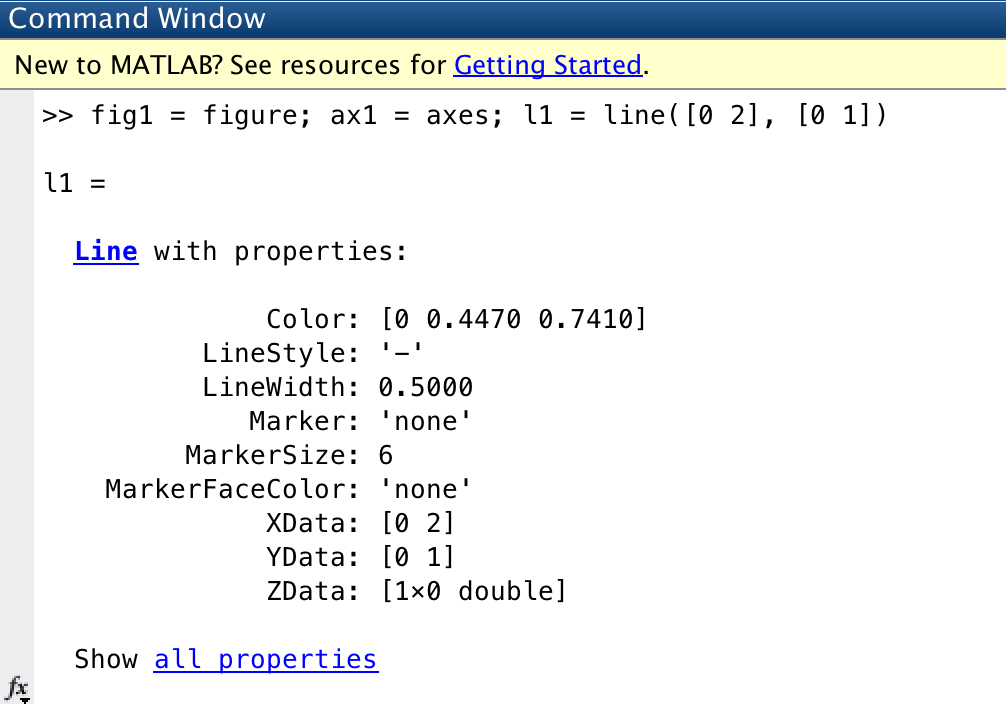
\includegraphics[width=0.475\textwidth]{graphics/NewFigAxLineCmdWinOut.png}
   \label{subfig:NewFigAxLineCmdWin}}
   \subfigure[ ]{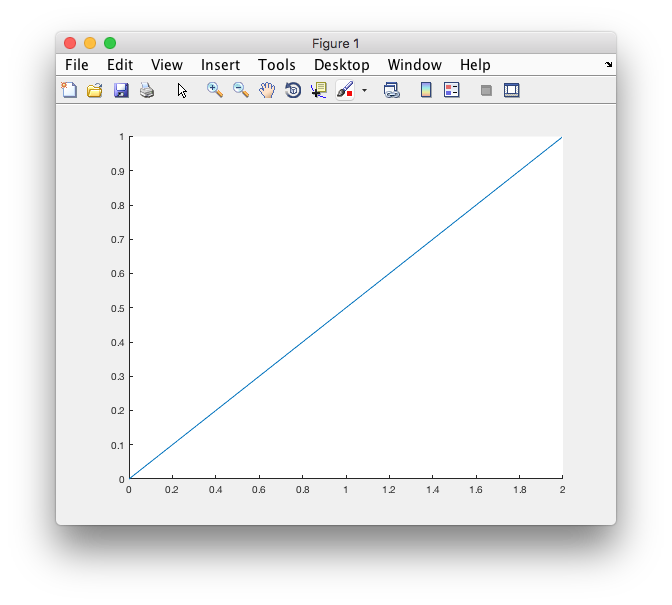
\includegraphics[width=0.475\textwidth]{graphics/NewFigAxLine.png} \label{subfig:NewFigAxLineWin}}
   \caption{Command Window output and graphical output of code of Listing \ref{NewFigAxLine}.}
   \label{fig:NewFigAxLine}
\end{figure}
% ^^^------------------------------------------------------------^^^
The \texttt{line} object \texttt{l1} has several properties, and many of these are suppressed in the Command Window output. Some important properties include \texttt{XData}, \texttt{YData}, \texttt{LineWidth}. Recall that we invoked the \texttt{line} constructor using \verb!line([0 2], [0 1])!. The first input array was a set of $x$-points and was stored in \texttt{l1.XData}. The second input array was a set of $y$-values, stored in \texttt{l1.YData}. Thus, the defining points for the \texttt{line} \texttt{l1} are given by making $(x,y)$ pairs from the values stored in these fields, and the line goes from $\mbox{(\texttt{XData(1)}, \texttt{YData(1)})}=(0,0)$ to $\mbox{(\texttt{XData(2)}, \texttt{YData(2)})}=(2,1)$.

% ============================================================
% ============================================================
\subsection{The Current \texttt{figure} and Current \texttt{axes} Objects}
% ============================================================
% ============================================================
Since \texttt{fig1} is the most recently-created \texttt{figure} object, it is referenced in MATLAB as the current figure. We can refer to it by the handle we created, \texttt{fig1}, or by the function \texttt{gcf} (get current figure), which returns a handle to the current \texttt{figure}. Similarly, \texttt{ax1} is the current \texttt{axes} object, which also may be referenced using \texttt{gca} (get current axes) or by \texttt{ax1}.

We can use the command \texttt{grid on} to toggle on grid lines for the current \texttt{axes}. Similarly, we can issue new plot commands, and they will generate new graphics objects as children of the current axes. We also can add $x$-axis and $y$-axis labels to the current \texttt{axes} by using the \texttt{xlabel} and \texttt{ylabel}. For example, consider Listing \ref{NewFigAxLinev01}:
% vvv------------------------------------------------------------vvv
\begin{lstlisting}[style=Matlab-editor,label=NewFigAxLinev01,caption={Command Window input to modify the \texttt{ax1}, the current axes object.}]
>> grid on; ax1.FontSize=16; xlbl = xlabel('$x$ (m)');  ylbl = ylabel('$y$ (m)'); xlbl.Interpreter='latex'; ylbl.Interpreter='latex';
\end{lstlisting}
% ^^^------------------------------------------------------------^^^
First, this input instructs MATLAB to display the grid; then, we enlarge the font for \texttt{ax1}; next, we define a variable \texttt{xlbl} as a handle for the \texttt{xlabel} object, which is assigned as a child of \texttt{ax1}. Similarly, \texttt{ylbl} is a handle for the \texttt{ylabel} object (also a child of \texttt{ax1}). The strings we provided within the \texttt{xlabel()} and \texttt{ylabel()} constructor methods enclose a symbol in dollar signs (\verb!$!). This is a fancy technique to make text appear as a mathematical expression as typeset in many textbooks. In order for this to work correctly, the appropriate object must have as it \texttt{Interpreter} property set to the value \texttt{'latex'}. We accomplish this is the remainder of the command in Listing \ref{NewFigAxLinev01}. The graphical result of Listing \ref{NewFigAxLinev01} is shown in Fig.\ \ref{subfig:NewFigAxLineWinv01}.
% vvv------------------------------------------------------------vvv
\begin{figure}[htbp] %  figure placement: here, top, bottom, or page
   \centering
   \subfigure[ ]{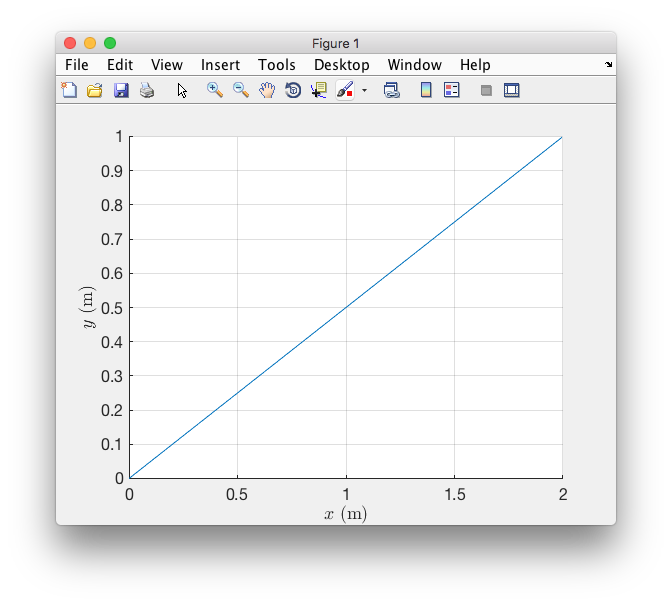
\includegraphics[width=0.475\textwidth]{graphics/NewFigAxLinev01.png} \label{subfig:NewFigAxLineWinv01}}
   \subfigure[ ]{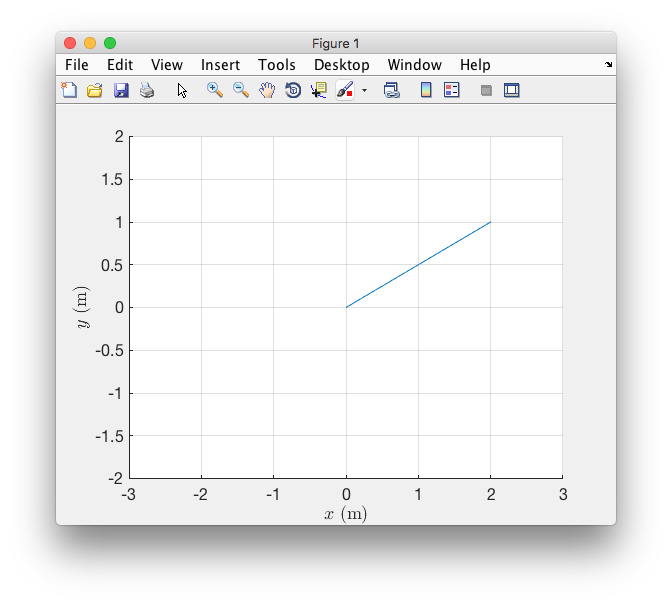
\includegraphics[width=0.475\textwidth]{graphics/NewFigAxLinev02axLims.png} \label{subfig:NewFigAxLineWinv02ScaledAx}}
   \caption{Command Window output and graphical output of code of Listing \ref{NewFigAxLine} [subfigure (a)] and Listing \ref{NewFigAxLinev01} [subfigure (b)]. In \ref{subfig:NewFigAxLineWinv01}, we have added a grid and axes labels. In \ref{subfig:NewFigAxLineWinv02ScaledAx}, we have adjusted the axes limits.}
   \label{fig:NewFigAxLine}
\end{figure}
% ^^^------------------------------------------------------------^^^
Compare Figs.\ \ref{subfig:NewFigAxLineWin} and \ref{subfig:NewFigAxLineWinv01} to see how we modified \texttt{ax1}.

% ============================================================
\subsubsection{Adjusting the Limits of the Current \texttt{axes}}
% ============================================================
It often is helpful to adjust the $x$- and $y$-limits of the current \texttt{axes}.  To do this, we can use the \texttt{xlim()} and \texttt{ylim()} functions. When invoked with no arguments, these functions return (get) a $1\times2$ array describing the $x$- or $y$-limits, but when invoked with a single $1\times2$ vector of the form \verb![vlo vhi]!, these functions set the applicable axes limits.
As an example, we set the axes limits to be $[-3, 3]$ in the $x$-direction and $[-2, 2]$ in the $y$-direction using the following command:
% vvv------------------------------------------------------------vvv
\begin{lstlisting}[style=Matlab-editor,label=NewFigAxLinevSetAxLim,caption={A Command Window input to set the axes limits for the current \texttt{axes} object.}]
>> xlim([-3 3]); ylim([-2 2])
\end{lstlisting}
% ^^^------------------------------------------------------------^^^
This creates a larger graphical context for the line segment we drew, as shown in Fig.\ \ref {subfig:NewFigAxLineWinv02ScaledAx}.

% ============================================================
% ============================================================
\subsection{Some Basic Graphic Types}
% ============================================================
% ============================================================

% ============================================================
\subsubsection{The \texttt{line} Class}
% ============================================================

We already have seen the \texttt{line} class, which we instantiated using the \texttt{line()} constructor method. To modify the line's end points, we can simply modify the \texttt{line} object's \texttt{XData} and \texttt{YData} properties. As an example, we can create a line using a script such as this \texttt{basicLine.m} script:
% vvv------------------------------------------------------------vvv
\begin{lstlisting}[style=Matlab-editor,label=basicLine,caption={Listing of the script \texttt{basicLine.m}.}]
% basicLine.m

a = 1; b = 2; c = 3; d = 4;
L0 = line([a b], [c d], 'LineWidth', 2);
\end{lstlisting}
% ^^^------------------------------------------------------------^^^
Upon running this script, we will have the \texttt{line} object \texttt{L0} saved in memory, and it can easily be seen that the \texttt{XData} property stores the vector \verb![1, 2]!, and that \texttt{YData} stores the vector \verb![3, 4]!,
% vvv------------------------------------------------------------vvv
\begin{lstlisting}[style=Matlab-editor,label=basicLineCheck,caption={A Command Window verification of the \texttt{XData} and \texttt{YData} properties of the \texttt{L0} object created in Listing \ref{basicLine}.}]
>> L0.XData

ans =

     1     2

>> L0.YData

ans =

     3     4
\end{lstlisting}
% ^^^------------------------------------------------------------^^^

Also, we can use the \texttt{plot()} command to specify \texttt{line} objects with two endpoints and many connected data points. To learn the syntax of the \texttt{plot()} command, either do an Internet search, or type \verb!doc plot! or \verb!help plot! in the MATLAB Command Window.

We can make several modifications to the \texttt{line} object by changing its properties. We list some important properties here:
\begin{itemize}
\item \texttt{XData}, \texttt{YData}, and \texttt{ZData} can be modified to change a 2D or 3D line object (yes, MATLAB can make 3D plots).
\item \texttt{LineWidth} can be used to change the thickness of the line.
\item \texttt{LineStyle} can be used to set the style of the line.
\item \texttt{Marker} can be used to specify a marker for data points.
\end{itemize}
To learn about the many options available to you, type \verb!doc line!.

% ============================================================
\subsubsection{The \texttt{patch} Class}
% ============================================================
A MATLAB \texttt{patch} draws a closed polygon with straight edges. The polygon is specified by specifying the $x$-, $y$-, and optional $z$ values of each vertex. The polygon is closed by connecting the last vertex to the first.

The basic syntax for the \texttt{patch} constructor is \texttt{patch(X,Y,C)}. This creates a polygon of $N$ points, where \texttt{X} is a $1\times N$ vector of $x$ values, $Y$ is a $1\times N$ vector of $y$ values, and \texttt{C} is a color specifier. The color specifier can be a string to specify a basic color, such as \verb!'r'!, \verb!'g'!,\verb!'b'!,\verb!'c'!,\verb!'m'!,\verb!'y'!,\verb!'w'!, or \verb!'k'!; or, \texttt{C} may be a $3$-element RGB (red-blue-green) triple specifying an arbitrary color. For example: \verb!C = [1, 0, 0]! specifies elementary red; \verb!C = [0, 1, 0]! specifies green; \verb!C = [0, 0, 1]! specifies blue; \verb!C = [0, 0, 0]! specifies black; and \verb!C = [1, 1, 1]! specifies white.

As an example, I provide the listing of a \texttt{basicPatch.m} script. The patch is defined in lines 3-7, and following lines of code provide formatting.
% vvv------------------------------------------------------------vvv
\begin{lstlisting}[style=Matlab-editor,label=basicPatch,caption={Listing of the script \texttt{basicPatch.m}.}]
% basicPatch.m

x = [-1 -1 1 1]; % specify x-values for vertices
y = [-1 1 1 -1]; % specify y-values for vertices
C = [0.75 0 0.75]; % specify a purple-ish color

newSquare = patch(x, y, C)
set(gca, 'FontName', 'Times', 'FontSize', 20); % format the current axes
grid on;

xlim([-3 3]); % adjust the x-limits of the axis
ylim([-3 3]); % adjust the x-limits of the axis

xlabel('$x$ (m)', 'Interpreter', 'latex') % add an x-label
ylabel('$y$ (m)', 'Interpreter', 'latex') % add a y-label
\end{lstlisting}
% ^^^------------------------------------------------------------^^^
The output of the \texttt{basicPatch.m} script is shown in Fig.\ \ref{fig:basicPatchOutput}.

% vvv------------------------------------------------------------vvv
\begin{figure}[htbp] %  figure placement: here, top, bottom, or page
   \centering
   \subfigure[ ]{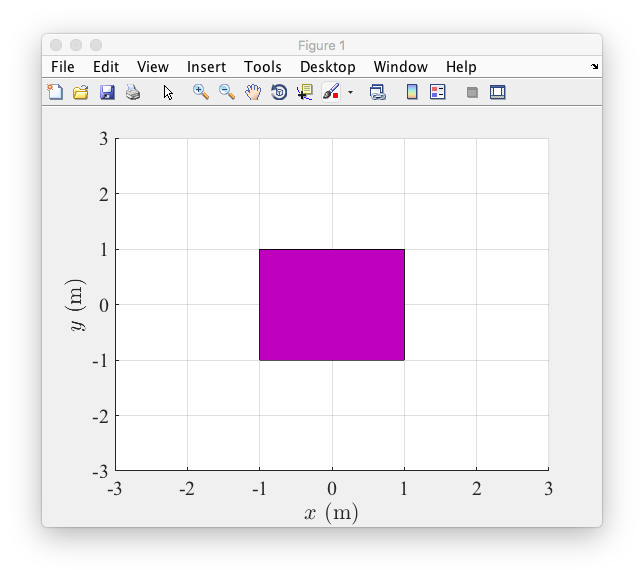
\includegraphics[width=0.475\textwidth]{graphics/basicPatchOutGraphical.png} \label{subfig:basicPatchOutputGraph}}
   \subfigure[ ]{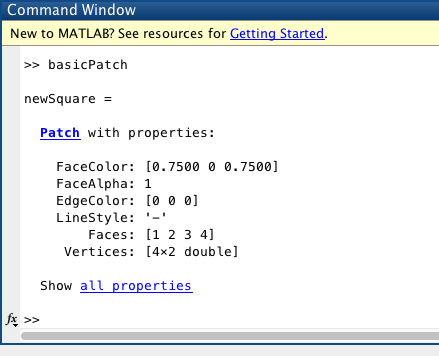
\includegraphics[width=0.475\textwidth]{graphics/basicPatchOutText.png} \label{subfig:basicPatchOutputText}}
   \caption{Graphical and Command Window output of the \texttt{basicPatch.m} script of Listing \ref{basicPatch}.}
   \label{fig:basicPatchOutput}
\end{figure}
% ^^^------------------------------------------------------------^^^

%The unsupressed output of Line 7 lists some properties of the \texttt{patch} object.
The \texttt{patch} object is centered at the origin in Fig.\ \ref{subfig:basicPatchOutputGraph}. An example of a simple modification to this is to translate the patch by the vector $(\Delta x, \Delta y)$. To do this, we define $\Delta x$ and $\Delta y$, and add these to the original \texttt{XData} and \texttt{YData} properties of the \texttt{newSquare} object. This can be done in the Command Window using the \texttt{set()} function:
% vvv------------------------------------------------------------vvv
\begin{lstlisting}[style=Matlab-editor,label=basicPatchDisplace,caption={A Command Window modification to the \texttt{patch} defined in Listing \ref{basicPatch}. Line 1 is used to specify the $x$- and $y$-components of the displacement. The displacement is then applied to the original \texttt{XData} and \texttt{YData} properties, and the result of the addition is the value component of a property-value pair in the \texttt{set()} function.}]
>> Dx = -2; Dy = 1.5;
>> set(newSquare, 'XData', newSquare.XData + Dx, 'YData', newSquare.YData + DY)
\end{lstlisting}
% ^^^------------------------------------------------------------^^^
The syntax here is \verb!set(obj, Prop1, Val1, Prop2, Val2, ...)!, where \texttt{obj} is the object we wish to modify, and we use property-value pairs to assign new object properties. The displaced \texttt{patch} object is displayed in Fig.\ \ref{fig:basicPatchDisplaced}. Similar modifications may be made to a \texttt{line}-class object.

% vvv------------------------------------------------------------vvv
\begin{figure}[htbp] %  figure placement: here, top, bottom, or page
   \centering
   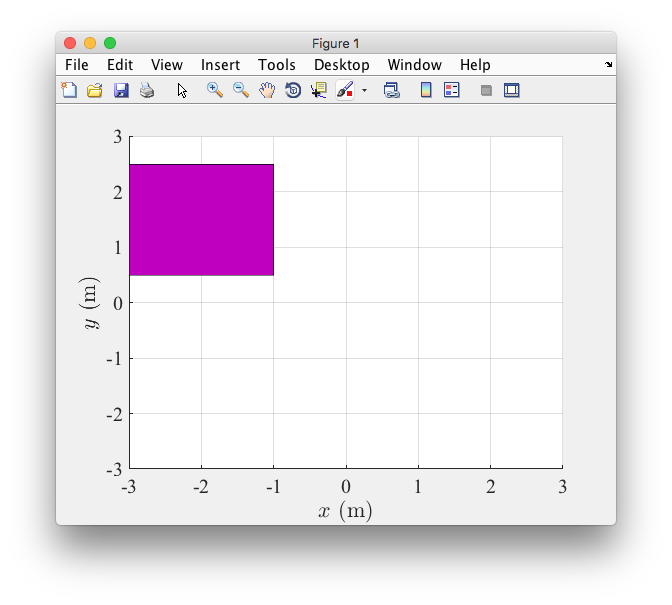
\includegraphics[width=0.475\textwidth]{graphics/basicPatchDisplaced.png}   
      \caption{The \texttt{patch} object created using \texttt{basicPatch.m} is modified by using the \texttt{set()} function using the code of Listing \ref{basicPatchDisplace}. The resulting \texttt{patch} no longer sits at the origin.}
\label{fig:basicPatchDisplaced}

\end{figure}
% ^^^------------------------------------------------------------^^^

For more information about the \texttt{patch} class, type \texttt{doc patch} in the MATLAB Command Window, or do an Internet search.